\documentclass[1p]{elsarticle_modified}
%\bibliographystyle{elsarticle-num}

%\usepackage[colorlinks]{hyperref}
%\usepackage{abbrmath_seonhwa} %\Abb, \Ascr, \Acal ,\Abf, \Afrak
\usepackage{amsfonts}
\usepackage{amssymb}
\usepackage{amsmath}
\usepackage{amsthm}
\usepackage{scalefnt}
\usepackage{amsbsy}
\usepackage{kotex}
\usepackage{caption}
\usepackage{subfig}
\usepackage{color}
\usepackage{graphicx}
\usepackage{xcolor} %% white, black, red, green, blue, cyan, magenta, yellow
\usepackage{float}
\usepackage{setspace}
\usepackage{hyperref}

\usepackage{tikz}
\usetikzlibrary{arrows}

\usepackage{multirow}
\usepackage{array} % fixed length table
\usepackage{hhline}

%%%%%%%%%%%%%%%%%%%%%
\makeatletter
\renewcommand*\env@matrix[1][\arraystretch]{%
	\edef\arraystretch{#1}%
	\hskip -\arraycolsep
	\let\@ifnextchar\new@ifnextchar
	\array{*\c@MaxMatrixCols c}}
\makeatother %https://tex.stackexchange.com/questions/14071/how-can-i-increase-the-line-spacing-in-a-matrix
%%%%%%%%%%%%%%%

\usepackage[normalem]{ulem}

\newcommand{\msout}[1]{\ifmmode\text{\sout{\ensuremath{#1}}}\else\sout{#1}\fi}
%SOURCE: \msout is \stkout macro in https://tex.stackexchange.com/questions/20609/strikeout-in-math-mode

\newcommand{\cancel}[1]{
	\ifmmode
	{\color{red}\msout{#1}}
	\else
	{\color{red}\sout{#1}}
	\fi
}

\newcommand{\add}[1]{
	{\color{blue}\uwave{#1}}
}

\newcommand{\replace}[2]{
	\ifmmode
	{\color{red}\msout{#1}}{\color{blue}\uwave{#2}}
	\else
	{\color{red}\sout{#1}}{\color{blue}\uwave{#2}}
	\fi
}

\newcommand{\Sol}{\mathcal{S}} %segment
\newcommand{\D}{D} %diagram
\newcommand{\A}{\mathcal{A}} %arc


%%%%%%%%%%%%%%%%%%%%%%%%%%%%%5 test

\def\sl{\operatorname{\textup{SL}}(2,\Cbb)}
\def\psl{\operatorname{\textup{PSL}}(2,\Cbb)}
\def\quan{\mkern 1mu \triangleright \mkern 1mu}

\theoremstyle{definition}
\newtheorem{thm}{Theorem}[section]
\newtheorem{prop}[thm]{Proposition}
\newtheorem{lem}[thm]{Lemma}
\newtheorem{ques}[thm]{Question}
\newtheorem{cor}[thm]{Corollary}
\newtheorem{defn}[thm]{Definition}
\newtheorem{exam}[thm]{Example}
\newtheorem{rmk}[thm]{Remark}
\newtheorem{alg}[thm]{Algorithm}

\newcommand{\I}{\sqrt{-1}}
\begin{document}

%\begin{frontmatter}
%
%\title{Boundary parabolic representations of knots up to 8 crossings}
%
%%% Group authors per affiliation:
%\author{Yunhi Cho} 
%\address{Department of Mathematics, University of Seoul, Seoul, Korea}
%\ead{yhcho@uos.ac.kr}
%
%
%\author{Seonhwa Kim} %\fnref{s_kim}}
%\address{Center for Geometry and Physics, Institute for Basic Science, Pohang, 37673, Korea}
%\ead{ryeona17@ibs.re.kr}
%
%\author{Hyuk Kim}
%\address{Department of Mathematical Sciences, Seoul National University, Seoul 08826, Korea}
%\ead{hyukkim@snu.ac.kr}
%
%\author{Seokbeom Yoon}
%\address{Department of Mathematical Sciences, Seoul National University, Seoul, 08826,  Korea}
%\ead{sbyoon15@snu.ac.kr}
%
%\begin{abstract}
%We find all boundary parabolic representation of knots up to 8 crossings.
%
%\end{abstract}
%\begin{keyword}
%    \MSC[2010] 57M25 
%\end{keyword}
%
%\end{frontmatter}

%\linenumbers
%\tableofcontents
%
\newcommand\colored[1]{\textcolor{white}{\rule[-0.35ex]{0.8em}{1.4ex}}\kern-0.8em\color{red} #1}%
%\newcommand\colored[1]{\textcolor{white}{ #1}\kern-2.17ex	\textcolor{white}{ #1}\kern-1.81ex	\textcolor{white}{ #1}\kern-2.15ex\color{red}#1	}

{\Large $\underline{12n_{0260}~(K12n_{0260})}$}

\setlength{\tabcolsep}{10pt}
\renewcommand{\arraystretch}{1.6}
\vspace{1cm}\begin{tabular}{m{100pt}>{\centering\arraybackslash}m{274pt}}
\multirow{5}{120pt}{
	\centering
	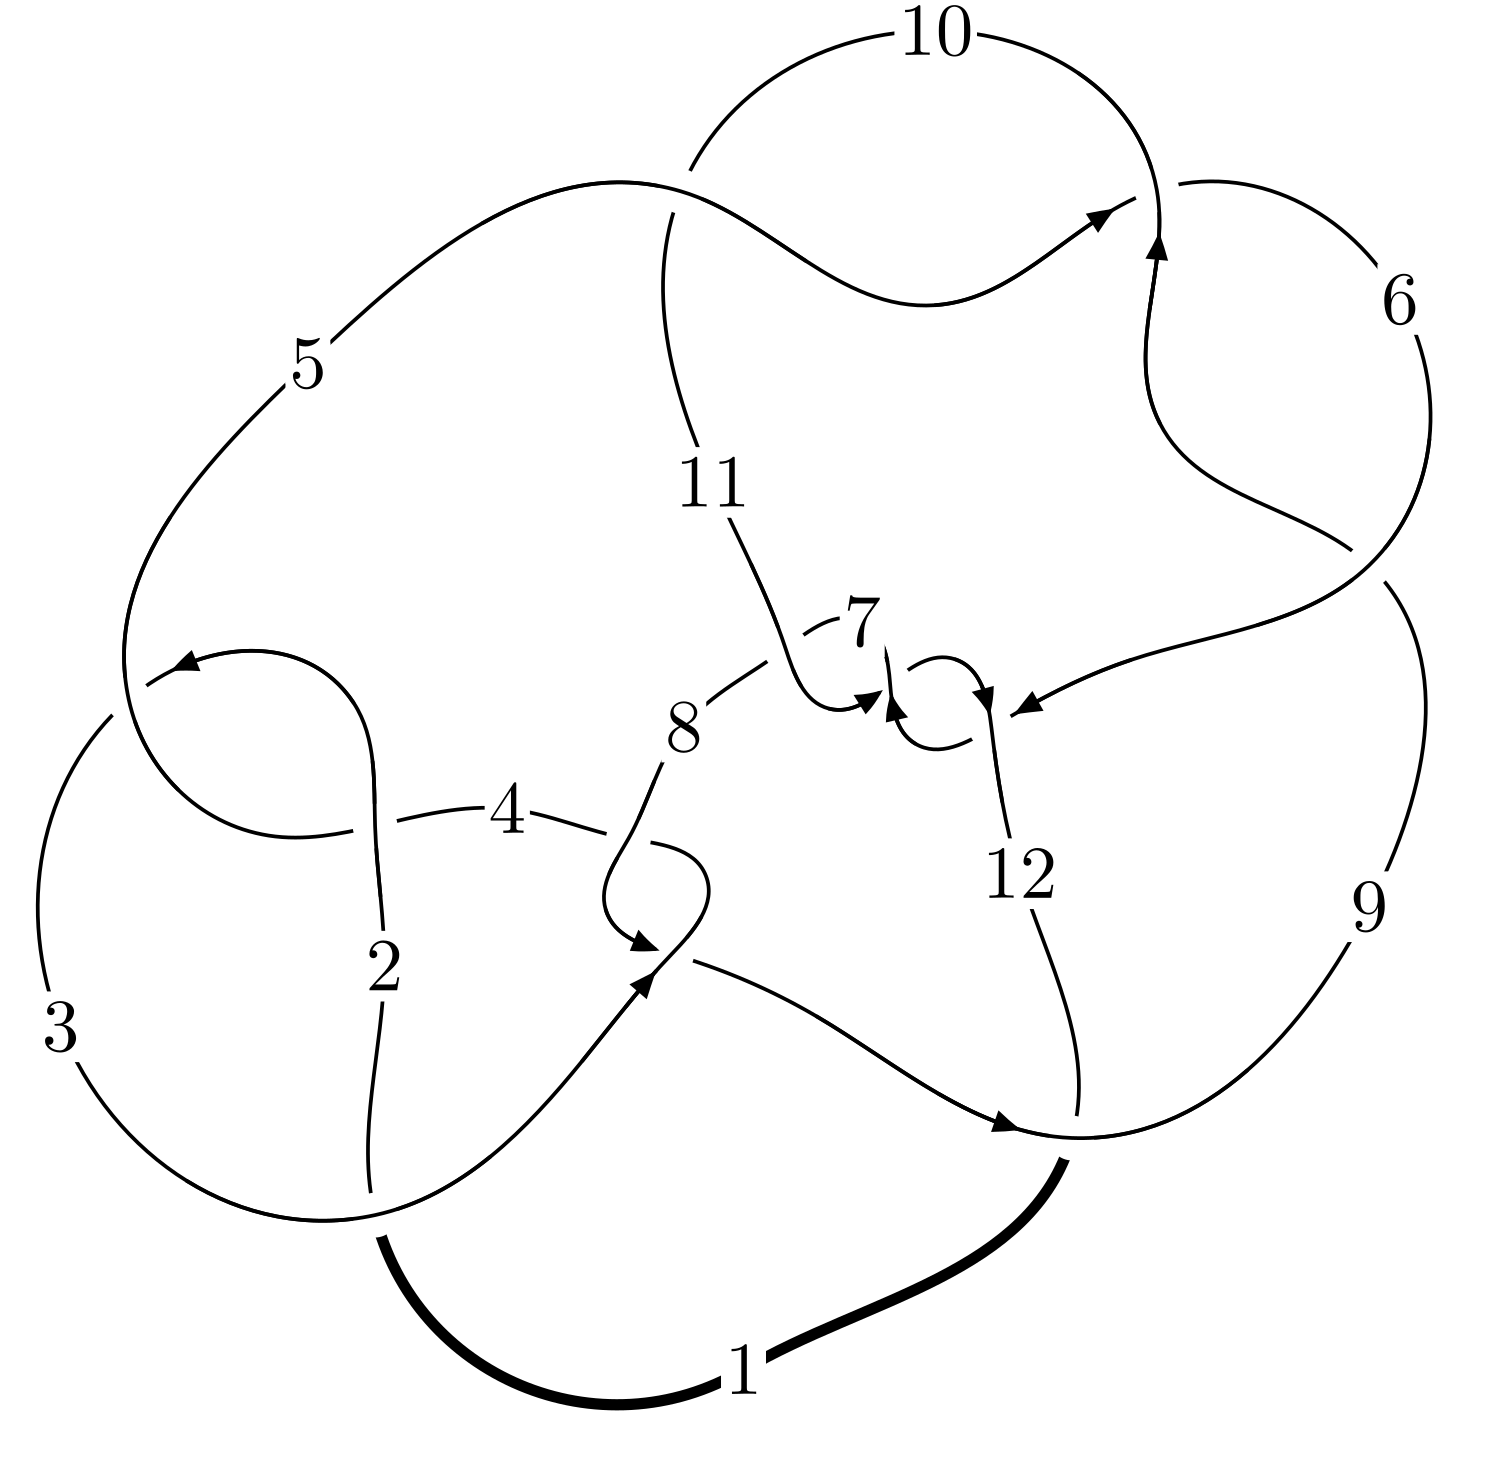
\includegraphics[width=112pt]{../../../GIT/diagram.site/Diagrams/png/2349_12n_0260.png}\\
\ \ \ A knot diagram\footnotemark}&
\allowdisplaybreaks
\textbf{Linearized knot diagam} \\
\cline{2-2}
 &
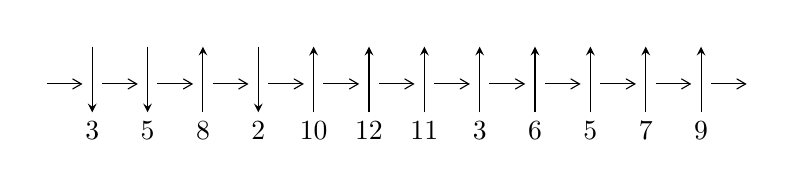
\begin{tikzpicture}[x=20pt, y=17pt]
	% nodes
	\node (C0) at (0, 0) {};
	\node (C1) at (1, 0) {};
	\node (C1U) at (1, +1) {};
	\node (C1D) at (1, -1) {3};

	\node (C2) at (2, 0) {};
	\node (C2U) at (2, +1) {};
	\node (C2D) at (2, -1) {5};

	\node (C3) at (3, 0) {};
	\node (C3U) at (3, +1) {};
	\node (C3D) at (3, -1) {8};

	\node (C4) at (4, 0) {};
	\node (C4U) at (4, +1) {};
	\node (C4D) at (4, -1) {2};

	\node (C5) at (5, 0) {};
	\node (C5U) at (5, +1) {};
	\node (C5D) at (5, -1) {10};

	\node (C6) at (6, 0) {};
	\node (C6U) at (6, +1) {};
	\node (C6D) at (6, -1) {12};

	\node (C7) at (7, 0) {};
	\node (C7U) at (7, +1) {};
	\node (C7D) at (7, -1) {11};

	\node (C8) at (8, 0) {};
	\node (C8U) at (8, +1) {};
	\node (C8D) at (8, -1) {3};

	\node (C9) at (9, 0) {};
	\node (C9U) at (9, +1) {};
	\node (C9D) at (9, -1) {6};

	\node (C10) at (10, 0) {};
	\node (C10U) at (10, +1) {};
	\node (C10D) at (10, -1) {5};

	\node (C11) at (11, 0) {};
	\node (C11U) at (11, +1) {};
	\node (C11D) at (11, -1) {7};

	\node (C12) at (12, 0) {};
	\node (C12U) at (12, +1) {};
	\node (C12D) at (12, -1) {9};
	\node (C13) at (13, 0) {};

	% arrows
	\draw[->,>={angle 60}]
	(C0) edge (C1) (C1) edge (C2) (C2) edge (C3) (C3) edge (C4) (C4) edge (C5) (C5) edge (C6) (C6) edge (C7) (C7) edge (C8) (C8) edge (C9) (C9) edge (C10) (C10) edge (C11) (C11) edge (C12) (C12) edge (C13) ;	\draw[->,>=stealth]
	(C1U) edge (C1D) (C2U) edge (C2D) (C3D) edge (C3U) (C4U) edge (C4D) (C5D) edge (C5U) (C6D) edge (C6U) (C7D) edge (C7U) (C8D) edge (C8U) (C9D) edge (C9U) (C10D) edge (C10U) (C11D) edge (C11U) (C12D) edge (C12U) ;
	\end{tikzpicture} \\
\hhline{~~} \\& 
\textbf{Solving Sequence} \\ \cline{2-2} 
 &
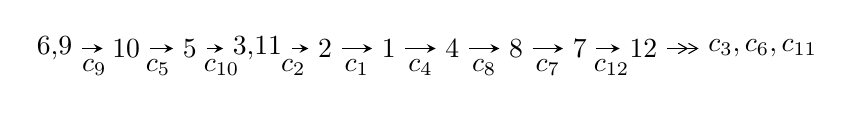
\begin{tikzpicture}[x=23pt, y=7pt]
	% node
	\node (A0) at (-1/8, 0) {6,9};
	\node (A1) at (1, 0) {10};
	\node (A2) at (2, 0) {5};
	\node (A3) at (49/16, 0) {3,11};
	\node (A4) at (33/8, 0) {2};
	\node (A5) at (41/8, 0) {1};
	\node (A6) at (49/8, 0) {4};
	\node (A7) at (57/8, 0) {8};
	\node (A8) at (65/8, 0) {7};
	\node (A9) at (73/8, 0) {12};
	\node (C1) at (1/2, -1) {$c_{9}$};
	\node (C2) at (3/2, -1) {$c_{5}$};
	\node (C3) at (5/2, -1) {$c_{10}$};
	\node (C4) at (29/8, -1) {$c_{2}$};
	\node (C5) at (37/8, -1) {$c_{1}$};
	\node (C6) at (45/8, -1) {$c_{4}$};
	\node (C7) at (53/8, -1) {$c_{8}$};
	\node (C8) at (61/8, -1) {$c_{7}$};
	\node (C9) at (69/8, -1) {$c_{12}$};
	\node (A10) at (11, 0) {$c_{3},c_{6},c_{11}$};

	% edge
	\draw[->,>=stealth]	
	(A0) edge (A1) (A1) edge (A2) (A2) edge (A3) (A3) edge (A4) (A4) edge (A5) (A5) edge (A6) (A6) edge (A7) (A7) edge (A8) (A8) edge (A9) ;
	\draw[->>,>={angle 60}]	
	(A9) edge (A10);
\end{tikzpicture} \\ 

\end{tabular} \\

\footnotetext{
The image of knot diagram is generated by the software ``\textbf{Draw programme}" developed by Andrew Bartholomew(\url{http://www.layer8.co.uk/maths/draw/index.htm\#Running-draw}), where we modified some parts for our purpose(\url{https://github.com/CATsTAILs/LinksPainter}).
}\phantom \\ \newline 
\centering \textbf{Ideals for irreducible components\footnotemark of $X_{\text{par}}$} 
 
\begin{align*}
I^u_{1}&=\langle 
-3 u^{10}+u^9-26 u^8+4 u^7-82 u^6+u^5-107 u^4-4 u^3-35 u^2+8 b+10 u+1,\\
\phantom{I^u_{1}}&\phantom{= \langle  }-21 u^{10}+7 u^9-186 u^8+20 u^7-594 u^6-33 u^5-785 u^4-48 u^3-265 u^2+32 a+162 u+15,\\
\phantom{I^u_{1}}&\phantom{= \langle  }u^{11}+9 u^9+2 u^8+30 u^7+11 u^6+44 u^5+15 u^4+21 u^3-3 u^2- u-1\rangle \\
I^u_{2}&=\langle 
b,\;- u^2+2 a- u-3,\;u^3+2 u-1\rangle \\
I^u_{3}&=\langle 
205 u^9-272 u^8+955 u^7-1446 u^6+1567 u^5-1260 u^4+1037 u^3+526 u^2+951 b+628 u+381,\\
\phantom{I^u_{3}}&\phantom{= \langle  }-190 u^9-235 u^8-514 u^7-585 u^6+728 u^5-711 u^4-590 u^3-3874 u^2+2853 a-1765 u-4737,\\
\phantom{I^u_{3}}&\phantom{= \langle  }u^{10}-2 u^9+7 u^8-12 u^7+19 u^6-21 u^5+23 u^4-11 u^3+16 u^2+9\rangle \\
I^u_{4}&=\langle 
b,\;u^3+a+u+1,\;u^4+u^3+2 u^2+2 u+1\rangle \\
I^u_{5}&=\langle 
- a u+2 b- a-2 u,\;a^2+a u+a-2 u,\;u^2+1\rangle \\
\\
\end{align*}
\raggedright * 5 irreducible components of $\dim_{\mathbb{C}}=0$, with total 32 representations.\\
\footnotetext{All coefficients of polynomials are rational numbers. But the coefficients are sometimes approximated in decimal forms when there is not enough margin.}
\newpage
\renewcommand{\arraystretch}{1}
\centering \section*{I. $I^u_{1}= \langle -3 u^{10}+u^9+\cdots+8 b+1,\;-21 u^{10}+7 u^9+\cdots+32 a+15,\;u^{11}+9 u^9+\cdots- u-1 \rangle$}
\flushleft \textbf{(i) Arc colorings}\\
\begin{tabular}{m{7pt} m{180pt} m{7pt} m{180pt} }
\flushright $a_{6}=$&$\begin{pmatrix}0\\u\end{pmatrix}$ \\
\flushright $a_{9}=$&$\begin{pmatrix}1\\0\end{pmatrix}$ \\
\flushright $a_{10}=$&$\begin{pmatrix}1\\- u^2\end{pmatrix}$ \\
\flushright $a_{5}=$&$\begin{pmatrix}- u\\u^3+u\end{pmatrix}$ \\
\flushright $a_{3}=$&$\begin{pmatrix}0.656250 u^{10}-0.218750 u^{9}+\cdots-5.06250 u-0.468750\\\frac{3}{8} u^{10}-\frac{1}{8} u^9+\cdots-\frac{5}{4} u-\frac{1}{8}\end{pmatrix}$ \\
\flushright $a_{11}=$&$\begin{pmatrix}u^2+1\\- u^4-2 u^2\end{pmatrix}$ \\
\flushright $a_{2}=$&$\begin{pmatrix}0.593750 u^{10}-0.0312500 u^{9}+\cdots-4.43750 u-0.781250\\\frac{1}{2} u^{10}+\frac{9}{2} u^8+\cdots+5 u^2-2 u\end{pmatrix}$ \\
\flushright $a_{1}=$&$\begin{pmatrix}\frac{1}{4} u^9+2 u^7+\cdots-\frac{1}{4} u-\frac{5}{4}\\\frac{1}{4} u^9+2 u^7+\cdots-\frac{1}{4} u-\frac{1}{4}\end{pmatrix}$ \\
\flushright $a_{4}=$&$\begin{pmatrix}0.281250 u^{10}-0.0937500 u^{9}+\cdots-4.81250 u+0.156250\\-\frac{3}{8} u^{10}+\frac{3}{8} u^9+\cdots-\frac{1}{2} u-\frac{1}{8}\end{pmatrix}$ \\
\flushright $a_{8}=$&$\begin{pmatrix}u^3+2 u\\-\frac{1}{4} u^{10}-2 u^8+\cdots+\frac{1}{4} u^2+\frac{5}{4} u\end{pmatrix}$ \\
\flushright $a_{7}=$&$\begin{pmatrix}u\\-\frac{1}{4} u^{10}-2 u^8+\cdots+\frac{1}{4} u^2+\frac{5}{4} u\end{pmatrix}$ \\
\flushright $a_{12}=$&$\begin{pmatrix}-1\\\frac{1}{4} u^9+2 u^7+\cdots-\frac{1}{4} u-\frac{1}{4}\end{pmatrix}$\\&\end{tabular}
\flushleft \textbf{(ii) Obstruction class $= -1$}\\~\\
\flushleft \textbf{(iii) Cusp Shapes $= \frac{39}{64} u^{10}+\frac{27}{64} u^9+\frac{175}{32} u^8+\frac{85}{16} u^7+\frac{619}{32} u^6+\frac{1419}{64} u^5+\frac{2147}{64} u^4+\frac{151}{4} u^3+\frac{1571}{64} u^2+\frac{633}{32} u+\frac{163}{64}$}\\~\\
\newpage\renewcommand{\arraystretch}{1}
\flushleft \textbf{(iv) u-Polynomials at the component}\newline \\
\begin{tabular}{m{50pt}|m{274pt}}
Crossings & \hspace{64pt}u-Polynomials at each crossing \\
\hline $$\begin{aligned}c_{1}\end{aligned}$$&$\begin{aligned}
&u^{11}+18 u^{10}+\cdots+1201 u+16
\end{aligned}$\\
\hline $$\begin{aligned}c_{2},c_{4}\end{aligned}$$&$\begin{aligned}
&u^{11}-4 u^{10}+\cdots+37 u-4
\end{aligned}$\\
\hline $$\begin{aligned}c_{3},c_{8}\end{aligned}$$&$\begin{aligned}
&u^{11}+3 u^{10}+\cdots+104 u-32
\end{aligned}$\\
\hline $$\begin{aligned}c_{5},c_{6},c_{7}\\c_{9},c_{10},c_{11}\end{aligned}$$&$\begin{aligned}
&u^{11}+9 u^9+2 u^8+30 u^7+11 u^6+44 u^5+15 u^4+21 u^3-3 u^2- u-1
\end{aligned}$\\
\hline $$\begin{aligned}c_{12}\end{aligned}$$&$\begin{aligned}
&u^{11}+13 u^9+2 u^8+50 u^7+25 u^6+61 u^5+79 u^4+71 u^3-7 u^2-4 u-4
\end{aligned}$\\
\hline
\end{tabular}\\~\\
\newpage\renewcommand{\arraystretch}{1}
\flushleft \textbf{(v) Riley Polynomials at the component}\newline \\
\begin{tabular}{m{50pt}|m{274pt}}
Crossings & \hspace{64pt}Riley Polynomials at each crossing \\
\hline $$\begin{aligned}c_{1}\end{aligned}$$&$\begin{aligned}
&y^{11}-14 y^{10}+\cdots+1302785 y-256
\end{aligned}$\\
\hline $$\begin{aligned}c_{2},c_{4}\end{aligned}$$&$\begin{aligned}
&y^{11}-18 y^{10}+\cdots+1201 y-16
\end{aligned}$\\
\hline $$\begin{aligned}c_{3},c_{8}\end{aligned}$$&$\begin{aligned}
&y^{11}+21 y^{10}+\cdots+6464 y-1024
\end{aligned}$\\
\hline $$\begin{aligned}c_{5},c_{6},c_{7}\\c_{9},c_{10},c_{11}\end{aligned}$$&$\begin{aligned}
&y^{11}+18 y^{10}+\cdots-5 y-1
\end{aligned}$\\
\hline $$\begin{aligned}c_{12}\end{aligned}$$&$\begin{aligned}
&y^{11}+26 y^{10}+\cdots-40 y-16
\end{aligned}$\\
\hline
\end{tabular}\\~\\
\newpage\flushleft \textbf{(vi) Complex Volumes and Cusp Shapes}
$$\begin{array}{c|c|c}  
\text{Solutions to }I^u_{1}& \I (\text{vol} + \sqrt{-1}CS) & \text{Cusp shape}\\
 \hline 
\begin{aligned}
u &= -0.405677 + 0.805557 I \\
a &= \phantom{-}0.760429 + 0.630050 I \\
b &= \phantom{-}0.11145 + 1.86194 I\end{aligned}
 & -11.46380 - 1.35185 I & \phantom{-}1.54505 + 5.14075 I \\ \hline\begin{aligned}
u &= -0.405677 - 0.805557 I \\
a &= \phantom{-}0.760429 - 0.630050 I \\
b &= \phantom{-}0.11145 - 1.86194 I\end{aligned}
 & -11.46380 + 1.35185 I & \phantom{-}1.54505 - 5.14075 I \\ \hline\begin{aligned}
u &= -0.23897 + 1.55675 I \\
a &= \phantom{-}0.230096 - 0.384371 I \\
b &= \phantom{-}1.033710 + 0.020727 I\end{aligned}
 & -10.53020 - 4.19214 I & \phantom{-}1.36233 + 0.44368 I \\ \hline\begin{aligned}
u &= -0.23897 - 1.55675 I \\
a &= \phantom{-}0.230096 + 0.384371 I \\
b &= \phantom{-}1.033710 - 0.020727 I\end{aligned}
 & -10.53020 + 4.19214 I & \phantom{-}1.36233 - 0.44368 I \\ \hline\begin{aligned}
u &= \phantom{-}0.375177\phantom{ +0.000000I} \\
a &= -0.576120\phantom{ +0.000000I} \\
b &= \phantom{-}0.341658\phantom{ +0.000000I}\end{aligned}
 & \phantom{-}0.611064\phantom{ +0.000000I} & \phantom{-}16.3080\phantom{ +0.000000I} \\ \hline\begin{aligned}
u &= -0.168597 + 0.298863 I \\
a &= -0.19001 - 2.05542 I \\
b &= -0.229927 - 0.652177 I\end{aligned}
 & -1.60266 - 0.72420 I & -1.00231 + 3.71560 I \\ \hline\begin{aligned}
u &= -0.168597 - 0.298863 I \\
a &= -0.19001 + 2.05542 I \\
b &= -0.229927 + 0.652177 I\end{aligned}
 & -1.60266 + 0.72420 I & -1.00231 - 3.71560 I \\ \hline\begin{aligned}
u &= \phantom{-}0.51296 + 1.70104 I \\
a &= \phantom{-}0.76568 - 1.38765 I \\
b &= -1.21043 - 2.42503 I\end{aligned}
 & \phantom{-}11.0221 + 10.7546 I & -1.36525 - 3.85022 I \\ \hline\begin{aligned}
u &= \phantom{-}0.51296 - 1.70104 I \\
a &= \phantom{-}0.76568 + 1.38765 I \\
b &= -1.21043 + 2.42503 I\end{aligned}
 & \phantom{-}11.0221 - 10.7546 I & -1.36525 + 3.85022 I \\ \hline\begin{aligned}
u &= \phantom{-}0.11269 + 1.88177 I \\
a &= -0.528135 + 1.174060 I \\
b &= -1.37564 + 2.29704 I\end{aligned}
 & -17.3399 + 2.6033 I & -1.56897 - 1.12618 I\\
 \hline 
 \end{array}$$\newpage$$\begin{array}{c|c|c}  
\text{Solutions to }I^u_{1}& \I (\text{vol} + \sqrt{-1}CS) & \text{Cusp shape}\\
 \hline 
\begin{aligned}
u &= \phantom{-}0.11269 - 1.88177 I \\
a &= -0.528135 - 1.174060 I \\
b &= -1.37564 - 2.29704 I\end{aligned}
 & -17.3399 - 2.6033 I & -1.56897 + 1.12618 I\\
 \hline 
 \end{array}$$\newpage\newpage\renewcommand{\arraystretch}{1}
\centering \section*{II. $I^u_{2}= \langle b,\;- u^2+2 a- u-3,\;u^3+2 u-1 \rangle$}
\flushleft \textbf{(i) Arc colorings}\\
\begin{tabular}{m{7pt} m{180pt} m{7pt} m{180pt} }
\flushright $a_{6}=$&$\begin{pmatrix}0\\u\end{pmatrix}$ \\
\flushright $a_{9}=$&$\begin{pmatrix}1\\0\end{pmatrix}$ \\
\flushright $a_{10}=$&$\begin{pmatrix}1\\- u^2\end{pmatrix}$ \\
\flushright $a_{5}=$&$\begin{pmatrix}- u\\- u+1\end{pmatrix}$ \\
\flushright $a_{3}=$&$\begin{pmatrix}\frac{1}{2} u^2+\frac{1}{2} u+\frac{3}{2}\\0\end{pmatrix}$ \\
\flushright $a_{11}=$&$\begin{pmatrix}u^2+1\\- u\end{pmatrix}$ \\
\flushright $a_{2}=$&$\begin{pmatrix}\frac{1}{2} u^2+\frac{3}{2} u+\frac{3}{2}\\u-1\end{pmatrix}$ \\
\flushright $a_{1}=$&$\begin{pmatrix}u\\u-1\end{pmatrix}$ \\
\flushright $a_{4}=$&$\begin{pmatrix}\frac{1}{2} u^2+\frac{1}{2} u+\frac{3}{2}\\0\end{pmatrix}$ \\
\flushright $a_{8}=$&$\begin{pmatrix}1\\0\end{pmatrix}$ \\
\flushright $a_{7}=$&$\begin{pmatrix}u\\u^2\end{pmatrix}$ \\
\flushright $a_{12}=$&$\begin{pmatrix}1\\u-1\end{pmatrix}$\\&\end{tabular}
\flushleft \textbf{(ii) Obstruction class $= 1$}\\~\\
\flushleft \textbf{(iii) Cusp Shapes $= \frac{7}{4} u^2+\frac{21}{4} u+\frac{9}{4}$}\\~\\
\newpage\renewcommand{\arraystretch}{1}
\flushleft \textbf{(iv) u-Polynomials at the component}\newline \\
\begin{tabular}{m{50pt}|m{274pt}}
Crossings & \hspace{64pt}u-Polynomials at each crossing \\
\hline $$\begin{aligned}c_{1},c_{2}\end{aligned}$$&$\begin{aligned}
&(u-1)^3
\end{aligned}$\\
\hline $$\begin{aligned}c_{3},c_{8}\end{aligned}$$&$\begin{aligned}
&u^3
\end{aligned}$\\
\hline $$\begin{aligned}c_{4}\end{aligned}$$&$\begin{aligned}
&(u+1)^3
\end{aligned}$\\
\hline $$\begin{aligned}c_{5},c_{6},c_{7}\end{aligned}$$&$\begin{aligned}
&u^3+2 u+1
\end{aligned}$\\
\hline $$\begin{aligned}c_{9},c_{10},c_{11}\end{aligned}$$&$\begin{aligned}
&u^3+2 u-1
\end{aligned}$\\
\hline $$\begin{aligned}c_{12}\end{aligned}$$&$\begin{aligned}
&u^3-3 u^2+5 u-2
\end{aligned}$\\
\hline
\end{tabular}\\~\\
\newpage\renewcommand{\arraystretch}{1}
\flushleft \textbf{(v) Riley Polynomials at the component}\newline \\
\begin{tabular}{m{50pt}|m{274pt}}
Crossings & \hspace{64pt}Riley Polynomials at each crossing \\
\hline $$\begin{aligned}c_{1},c_{2},c_{4}\end{aligned}$$&$\begin{aligned}
&(y-1)^3
\end{aligned}$\\
\hline $$\begin{aligned}c_{3},c_{8}\end{aligned}$$&$\begin{aligned}
&y^3
\end{aligned}$\\
\hline $$\begin{aligned}c_{5},c_{6},c_{7}\\c_{9},c_{10},c_{11}\end{aligned}$$&$\begin{aligned}
&y^3+4 y^2+4 y-1
\end{aligned}$\\
\hline $$\begin{aligned}c_{12}\end{aligned}$$&$\begin{aligned}
&y^3+y^2+13 y-4
\end{aligned}$\\
\hline
\end{tabular}\\~\\
\newpage\flushleft \textbf{(vi) Complex Volumes and Cusp Shapes}
$$\begin{array}{c|c|c}  
\text{Solutions to }I^u_{2}& \I (\text{vol} + \sqrt{-1}CS) & \text{Cusp shape}\\
 \hline 
\begin{aligned}
u &= -0.22670 + 1.46771 I \\
a &= \phantom{-}0.335258 + 0.401127 I \\
b &= \phantom{-0.000000 } 0\end{aligned}
 & -11.08570 - 5.13794 I & -2.62004 + 6.54094 I \\ \hline\begin{aligned}
u &= -0.22670 - 1.46771 I \\
a &= \phantom{-}0.335258 - 0.401127 I \\
b &= \phantom{-0.000000 } 0\end{aligned}
 & -11.08570 + 5.13794 I & -2.62004 - 6.54094 I \\ \hline\begin{aligned}
u &= \phantom{-}0.453398\phantom{ +0.000000I} \\
a &= \phantom{-}1.82948\phantom{ +0.000000I} \\
b &= \phantom{-0.000000 } 0\end{aligned}
 & -0.857735\phantom{ +0.000000I} & \phantom{-}4.99010\phantom{ +0.000000I}\\
 \hline 
 \end{array}$$\newpage\newpage\renewcommand{\arraystretch}{1}
\centering \section*{III. $I^u_{3}= \langle 205 u^9-272 u^8+\cdots+951 b+381,\;-190 u^9-235 u^8+\cdots+2853 a-4737,\;u^{10}-2 u^9+\cdots+16 u^2+9 \rangle$}
\flushleft \textbf{(i) Arc colorings}\\
\begin{tabular}{m{7pt} m{180pt} m{7pt} m{180pt} }
\flushright $a_{6}=$&$\begin{pmatrix}0\\u\end{pmatrix}$ \\
\flushright $a_{9}=$&$\begin{pmatrix}1\\0\end{pmatrix}$ \\
\flushright $a_{10}=$&$\begin{pmatrix}1\\- u^2\end{pmatrix}$ \\
\flushright $a_{5}=$&$\begin{pmatrix}- u\\u^3+u\end{pmatrix}$ \\
\flushright $a_{3}=$&$\begin{pmatrix}0.0665966 u^{9}+0.0823694 u^{8}+\cdots+0.618647 u+1.66036\\-0.215563 u^{9}+0.286015 u^{8}+\cdots-0.660358 u-0.400631\end{pmatrix}$ \\
\flushright $a_{11}=$&$\begin{pmatrix}u^2+1\\- u^4-2 u^2\end{pmatrix}$ \\
\flushright $a_{2}=$&$\begin{pmatrix}0.0476691 u^{9}+0.322117 u^{8}+\cdots+0.653347 u+2.95689\\-0.376446 u^{9}+0.323870 u^{8}+\cdots-0.865405 u+0.119874\end{pmatrix}$ \\
\flushright $a_{1}=$&$\begin{pmatrix}-0.174553 u^{9}+0.433228 u^{8}+\cdots-1.23554 u+1.62355\\-0.126183 u^{9}+0.264984 u^{8}+\cdots-0.435331 u-0.356467\end{pmatrix}$ \\
\flushright $a_{4}=$&$\begin{pmatrix}-0.198738 u^{9}+0.850683 u^{8}+\cdots+0.197687 u+3.44690\\-0.164038 u^{9}+0.744479 u^{8}+\cdots-2.36593 u-0.763407\end{pmatrix}$ \\
\flushright $a_{8}=$&$\begin{pmatrix}0.123729 u^{9}-0.0487206 u^{8}+\cdots+1.42131 u+1.13565\\0.0357518 u^{9}-0.00841220 u^{8}+\cdots-0.509989 u+0.217666\end{pmatrix}$ \\
\flushright $a_{7}=$&$\begin{pmatrix}0.182615 u^{9}-0.239047 u^{8}+\cdots+2.75780 u+0.435331\\-0.0588854 u^{9}+0.190326 u^{8}+\cdots+0.663512 u+0.700315\end{pmatrix}$ \\
\flushright $a_{12}=$&$\begin{pmatrix}-0.0483701 u^{9}+0.168244 u^{8}+\cdots-0.800210 u+1.98002\\-0.126183 u^{9}+0.264984 u^{8}+\cdots-0.435331 u-0.356467\end{pmatrix}$\\&\end{tabular}
\flushleft \textbf{(ii) Obstruction class $= -1$}\\~\\
\flushleft \textbf{(iii) Cusp Shapes $= \frac{39}{317} u^9+\frac{140}{317} u^8-\frac{58}{317} u^7+\frac{362}{317} u^6-\frac{373}{317} u^5-\frac{116}{317} u^4+\frac{1289}{317} u^3-\frac{653}{317} u^2+\frac{1355}{317} u+\frac{1291}{317}$}\\~\\
\newpage\renewcommand{\arraystretch}{1}
\flushleft \textbf{(iv) u-Polynomials at the component}\newline \\
\begin{tabular}{m{50pt}|m{274pt}}
Crossings & \hspace{64pt}u-Polynomials at each crossing \\
\hline $$\begin{aligned}c_{1}\end{aligned}$$&$\begin{aligned}
&(u^5+11 u^4+37 u^3+30 u^2-12 u+1)^2
\end{aligned}$\\
\hline $$\begin{aligned}c_{2},c_{4}\end{aligned}$$&$\begin{aligned}
&(u^5-3 u^4- u^3+6 u^2+1)^2
\end{aligned}$\\
\hline $$\begin{aligned}c_{3},c_{8}\end{aligned}$$&$\begin{aligned}
&(u^5- u^4+8 u^3- u^2-4 u-4)^2
\end{aligned}$\\
\hline $$\begin{aligned}c_{5},c_{6},c_{7}\\c_{9},c_{10},c_{11}\end{aligned}$$&$\begin{aligned}
&u^{10}-2 u^9+7 u^8-12 u^7+19 u^6-21 u^5+23 u^4-11 u^3+16 u^2+9
\end{aligned}$\\
\hline $$\begin{aligned}c_{12}\end{aligned}$$&$\begin{aligned}
&(u^5+6 u^3+u-1)^2
\end{aligned}$\\
\hline
\end{tabular}\\~\\
\newpage\renewcommand{\arraystretch}{1}
\flushleft \textbf{(v) Riley Polynomials at the component}\newline \\
\begin{tabular}{m{50pt}|m{274pt}}
Crossings & \hspace{64pt}Riley Polynomials at each crossing \\
\hline $$\begin{aligned}c_{1}\end{aligned}$$&$\begin{aligned}
&(y^5-47 y^4+685 y^3-1810 y^2+84 y-1)^2
\end{aligned}$\\
\hline $$\begin{aligned}c_{2},c_{4}\end{aligned}$$&$\begin{aligned}
&(y^5-11 y^4+37 y^3-30 y^2-12 y-1)^2
\end{aligned}$\\
\hline $$\begin{aligned}c_{3},c_{8}\end{aligned}$$&$\begin{aligned}
&(y^5+15 y^4+54 y^3-73 y^2+8 y-16)^2
\end{aligned}$\\
\hline $$\begin{aligned}c_{5},c_{6},c_{7}\\c_{9},c_{10},c_{11}\end{aligned}$$&$\begin{aligned}
&y^{10}+10 y^9+\cdots+288 y+81
\end{aligned}$\\
\hline $$\begin{aligned}c_{12}\end{aligned}$$&$\begin{aligned}
&(y^5+12 y^4+38 y^3+12 y^2+y-1)^2
\end{aligned}$\\
\hline
\end{tabular}\\~\\
\newpage\flushleft \textbf{(vi) Complex Volumes and Cusp Shapes}
$$\begin{array}{c|c|c}  
\text{Solutions to }I^u_{3}& \I (\text{vol} + \sqrt{-1}CS) & \text{Cusp shape}\\
 \hline 
\begin{aligned}
u &= \phantom{-}0.334233 + 1.155480 I \\
a &= -1.03102 + 1.25338 I \\
b &= \phantom{-}1.04912\phantom{ +0.000000I}\end{aligned}
 & -5.84264\phantom{ +0.000000I} &                  -6
-0.349607 + 0. 10   I\phantom{ +0.000000I} \\ \hline\begin{aligned}
u &= \phantom{-}0.334233 - 1.155480 I \\
a &= -1.03102 - 1.25338 I \\
b &= \phantom{-}1.04912\phantom{ +0.000000I}\end{aligned}
 & -5.84264\phantom{ +0.000000I} &                  -6
-0.349607 + 0. 10   I\phantom{ +0.000000I} \\ \hline\begin{aligned}
u &= -0.447614 + 0.607198 I \\
a &= \phantom{-}1.181370 - 0.198963 I \\
b &= -0.465884 + 0.485496 I\end{aligned}
 & -3.23236 - 1.37362 I & \phantom{-}4.45374 + 4.59823 I \\ \hline\begin{aligned}
u &= -0.447614 - 0.607198 I \\
a &= \phantom{-}1.181370 + 0.198963 I \\
b &= -0.465884 - 0.485496 I\end{aligned}
 & -3.23236 + 1.37362 I & \phantom{-}4.45374 - 4.59823 I \\ \hline\begin{aligned}
u &= \phantom{-}0.011167 + 1.262230 I \\
a &= -0.223398 - 0.807514 I \\
b &= -0.465884 - 0.485496 I\end{aligned}
 & -3.23236 + 1.37362 I & \phantom{-}4.45374 - 4.59823 I \\ \hline\begin{aligned}
u &= \phantom{-}0.011167 - 1.262230 I \\
a &= -0.223398 + 0.807514 I \\
b &= -0.465884 + 0.485496 I\end{aligned}
 & -3.23236 - 1.37362 I & \phantom{-}4.45374 + 4.59823 I \\ \hline\begin{aligned}
u &= \phantom{-}1.28009 + 0.69443 I \\
a &= -0.932756 - 0.175792 I \\
b &= \phantom{-}0.44133 + 2.86818 I\end{aligned}
 & \phantom{-}18.4907 + 4.0569 I & -0.27894 - 1.95729 I \\ \hline\begin{aligned}
u &= \phantom{-}1.28009 - 0.69443 I \\
a &= -0.932756 + 0.175792 I \\
b &= \phantom{-}0.44133 - 2.86818 I\end{aligned}
 & \phantom{-}18.4907 - 4.0569 I & -0.27894 + 1.95729 I \\ \hline\begin{aligned}
u &= -0.17787 + 1.78975 I \\
a &= -0.32754 - 1.78671 I \\
b &= \phantom{-}0.44133 - 2.86818 I\end{aligned}
 & \phantom{-}18.4907 - 4.0569 I & -0.27894 + 1.95729 I \\ \hline\begin{aligned}
u &= -0.17787 - 1.78975 I \\
a &= -0.32754 + 1.78671 I \\
b &= \phantom{-}0.44133 + 2.86818 I\end{aligned}
 & \phantom{-}18.4907 + 4.0569 I & -0.27894 - 1.95729 I\\
 \hline 
 \end{array}$$\newpage\newpage\renewcommand{\arraystretch}{1}
\centering \section*{IV. $I^u_{4}= \langle b,\;u^3+a+u+1,\;u^4+u^3+2 u^2+2 u+1 \rangle$}
\flushleft \textbf{(i) Arc colorings}\\
\begin{tabular}{m{7pt} m{180pt} m{7pt} m{180pt} }
\flushright $a_{6}=$&$\begin{pmatrix}0\\u\end{pmatrix}$ \\
\flushright $a_{9}=$&$\begin{pmatrix}1\\0\end{pmatrix}$ \\
\flushright $a_{10}=$&$\begin{pmatrix}1\\- u^2\end{pmatrix}$ \\
\flushright $a_{5}=$&$\begin{pmatrix}- u\\u^3+u\end{pmatrix}$ \\
\flushright $a_{3}=$&$\begin{pmatrix}- u^3- u-1\\0\end{pmatrix}$ \\
\flushright $a_{11}=$&$\begin{pmatrix}u^2+1\\u^3+2 u+1\end{pmatrix}$ \\
\flushright $a_{2}=$&$\begin{pmatrix}- u^3-1\\- u^3- u\end{pmatrix}$ \\
\flushright $a_{1}=$&$\begin{pmatrix}u\\- u^3- u\end{pmatrix}$ \\
\flushright $a_{4}=$&$\begin{pmatrix}- u^3- u-1\\0\end{pmatrix}$ \\
\flushright $a_{8}=$&$\begin{pmatrix}1\\0\end{pmatrix}$ \\
\flushright $a_{7}=$&$\begin{pmatrix}2 u^3+u^2+3 u+3\\- u^3- u^2- u-2\end{pmatrix}$ \\
\flushright $a_{12}=$&$\begin{pmatrix}u^3+2 u\\- u^3- u\end{pmatrix}$\\&\end{tabular}
\flushleft \textbf{(ii) Obstruction class $= 1$}\\~\\
\flushleft \textbf{(iii) Cusp Shapes $= 4 u^3+4 u+3$}\\~\\
\newpage\renewcommand{\arraystretch}{1}
\flushleft \textbf{(iv) u-Polynomials at the component}\newline \\
\begin{tabular}{m{50pt}|m{274pt}}
Crossings & \hspace{64pt}u-Polynomials at each crossing \\
\hline $$\begin{aligned}c_{1},c_{2}\end{aligned}$$&$\begin{aligned}
&(u-1)^4
\end{aligned}$\\
\hline $$\begin{aligned}c_{3},c_{8}\end{aligned}$$&$\begin{aligned}
&u^4
\end{aligned}$\\
\hline $$\begin{aligned}c_{4}\end{aligned}$$&$\begin{aligned}
&(u+1)^4
\end{aligned}$\\
\hline $$\begin{aligned}c_{5},c_{6},c_{7}\end{aligned}$$&$\begin{aligned}
&u^4- u^3+2 u^2-2 u+1
\end{aligned}$\\
\hline $$\begin{aligned}c_{9},c_{10},c_{11}\end{aligned}$$&$\begin{aligned}
&u^4+u^3+2 u^2+2 u+1
\end{aligned}$\\
\hline $$\begin{aligned}c_{12}\end{aligned}$$&$\begin{aligned}
&(u^2+u+1)^2
\end{aligned}$\\
\hline
\end{tabular}\\~\\
\newpage\renewcommand{\arraystretch}{1}
\flushleft \textbf{(v) Riley Polynomials at the component}\newline \\
\begin{tabular}{m{50pt}|m{274pt}}
Crossings & \hspace{64pt}Riley Polynomials at each crossing \\
\hline $$\begin{aligned}c_{1},c_{2},c_{4}\end{aligned}$$&$\begin{aligned}
&(y-1)^4
\end{aligned}$\\
\hline $$\begin{aligned}c_{3},c_{8}\end{aligned}$$&$\begin{aligned}
&y^4
\end{aligned}$\\
\hline $$\begin{aligned}c_{5},c_{6},c_{7}\\c_{9},c_{10},c_{11}\end{aligned}$$&$\begin{aligned}
&y^4+3 y^3+2 y^2+1
\end{aligned}$\\
\hline $$\begin{aligned}c_{12}\end{aligned}$$&$\begin{aligned}
&(y^2+y+1)^2
\end{aligned}$\\
\hline
\end{tabular}\\~\\
\newpage\flushleft \textbf{(vi) Complex Volumes and Cusp Shapes}
$$\begin{array}{c|c|c}  
\text{Solutions to }I^u_{4}& \I (\text{vol} + \sqrt{-1}CS) & \text{Cusp shape}\\
 \hline 
\begin{aligned}
u &= -0.621744 + 0.440597 I \\
a &= -0.500000 - 0.866025 I \\
b &= \phantom{-0.000000 } 0\end{aligned}
 & -4.93480 - 2.02988 I & \phantom{-}1.0000 + 3.46410 I \\ \hline\begin{aligned}
u &= -0.621744 - 0.440597 I \\
a &= -0.500000 + 0.866025 I \\
b &= \phantom{-0.000000 } 0\end{aligned}
 & -4.93480 + 2.02988 I & \phantom{-}1.0000 - 3.46410 I \\ \hline\begin{aligned}
u &= \phantom{-}0.121744 + 1.306620 I \\
a &= -0.500000 + 0.866025 I \\
b &= \phantom{-0.000000 } 0\end{aligned}
 & -4.93480 + 2.02988 I & \phantom{-}1.00000 - 3.46410 I \\ \hline\begin{aligned}
u &= \phantom{-}0.121744 - 1.306620 I \\
a &= -0.500000 - 0.866025 I \\
b &= \phantom{-0.000000 } 0\end{aligned}
 & -4.93480 - 2.02988 I & \phantom{-}1.00000 + 3.46410 I\\
 \hline 
 \end{array}$$\newpage\newpage\renewcommand{\arraystretch}{1}
\centering \section*{V. $I^u_{5}= \langle - a u+2 b- a-2 u,\;a^2+a u+a-2 u,\;u^2+1 \rangle$}
\flushleft \textbf{(i) Arc colorings}\\
\begin{tabular}{m{7pt} m{180pt} m{7pt} m{180pt} }
\flushright $a_{6}=$&$\begin{pmatrix}0\\u\end{pmatrix}$ \\
\flushright $a_{9}=$&$\begin{pmatrix}1\\0\end{pmatrix}$ \\
\flushright $a_{10}=$&$\begin{pmatrix}1\\1\end{pmatrix}$ \\
\flushright $a_{5}=$&$\begin{pmatrix}- u\\0\end{pmatrix}$ \\
\flushright $a_{3}=$&$\begin{pmatrix}a\\\frac{1}{2} a u+\frac{1}{2} a+u\end{pmatrix}$ \\
\flushright $a_{11}=$&$\begin{pmatrix}0\\1\end{pmatrix}$ \\
\flushright $a_{2}=$&$\begin{pmatrix}-\frac{1}{2} a u+\frac{1}{2} a- u\\\frac{1}{2} a u+\frac{1}{2} a+u\end{pmatrix}$ \\
\flushright $a_{1}=$&$\begin{pmatrix}-\frac{1}{2} a u-\frac{1}{2} a-2 u-1\\-\frac{1}{2} a u-\frac{1}{2} a-2 u\end{pmatrix}$ \\
\flushright $a_{4}=$&$\begin{pmatrix}\frac{1}{2} a u+\frac{1}{2} a-1\\-\frac{1}{2} a u-\frac{1}{2} a-2 u\end{pmatrix}$ \\
\flushright $a_{8}=$&$\begin{pmatrix}u\\\frac{1}{2} a u-\frac{1}{2} a-2\end{pmatrix}$ \\
\flushright $a_{7}=$&$\begin{pmatrix}u\\\frac{1}{2} a u-\frac{1}{2} a+u-2\end{pmatrix}$ \\
\flushright $a_{12}=$&$\begin{pmatrix}-1\\-\frac{1}{2} a u-\frac{1}{2} a-2 u\end{pmatrix}$\\&\end{tabular}
\flushleft \textbf{(ii) Obstruction class $= 1$}\\~\\
\flushleft \textbf{(iii) Cusp Shapes $= -4$}\\~\\
\newpage\renewcommand{\arraystretch}{1}
\flushleft \textbf{(iv) u-Polynomials at the component}\newline \\
\begin{tabular}{m{50pt}|m{274pt}}
Crossings & \hspace{64pt}u-Polynomials at each crossing \\
\hline $$\begin{aligned}c_{1}\end{aligned}$$&$\begin{aligned}
&(u^2-3 u+1)^2
\end{aligned}$\\
\hline $$\begin{aligned}c_{2}\end{aligned}$$&$\begin{aligned}
&(u^2+u-1)^2
\end{aligned}$\\
\hline $$\begin{aligned}c_{3},c_{8}\end{aligned}$$&$\begin{aligned}
&u^4+3 u^2+1
\end{aligned}$\\
\hline $$\begin{aligned}c_{4}\end{aligned}$$&$\begin{aligned}
&(u^2- u-1)^2
\end{aligned}$\\
\hline $$\begin{aligned}c_{5},c_{6},c_{7}\\c_{9},c_{10},c_{11}\end{aligned}$$&$\begin{aligned}
&(u^2+1)^2
\end{aligned}$\\
\hline $$\begin{aligned}c_{12}\end{aligned}$$&$\begin{aligned}
&u^4+7 u^2+1
\end{aligned}$\\
\hline
\end{tabular}\\~\\
\newpage\renewcommand{\arraystretch}{1}
\flushleft \textbf{(v) Riley Polynomials at the component}\newline \\
\begin{tabular}{m{50pt}|m{274pt}}
Crossings & \hspace{64pt}Riley Polynomials at each crossing \\
\hline $$\begin{aligned}c_{1}\end{aligned}$$&$\begin{aligned}
&(y^2-7 y+1)^2
\end{aligned}$\\
\hline $$\begin{aligned}c_{2},c_{4}\end{aligned}$$&$\begin{aligned}
&(y^2-3 y+1)^2
\end{aligned}$\\
\hline $$\begin{aligned}c_{3},c_{8}\end{aligned}$$&$\begin{aligned}
&(y^2+3 y+1)^2
\end{aligned}$\\
\hline $$\begin{aligned}c_{5},c_{6},c_{7}\\c_{9},c_{10},c_{11}\end{aligned}$$&$\begin{aligned}
&(y+1)^4
\end{aligned}$\\
\hline $$\begin{aligned}c_{12}\end{aligned}$$&$\begin{aligned}
&(y^2+7 y+1)^2
\end{aligned}$\\
\hline
\end{tabular}\\~\\
\newpage\flushleft \textbf{(vi) Complex Volumes and Cusp Shapes}
$$\begin{array}{c|c|c}  
\text{Solutions to }I^u_{5}& \I (\text{vol} + \sqrt{-1}CS) & \text{Cusp shape}\\
 \hline 
\begin{aligned}
u &= \phantom{-0.000000 -}1.000000 I \\
a &= \phantom{-}0.618034 + 0.618034 I \\
b &= \phantom{-0.000000 -}1.61803 I\end{aligned}
 & -12.1725\phantom{ +0.000000I} & -4.00000\phantom{ +0.000000I} \\ \hline\begin{aligned}
u &= \phantom{-0.000000 -}1.000000 I \\
a &= -1.61803 - 1.61803 I \\
b &= \phantom{-0.000000 } -0.618034 I\end{aligned}
 & -4.27683\phantom{ +0.000000I} & -4.00000\phantom{ +0.000000I} \\ \hline\begin{aligned}
u &= \phantom{-0.000000 } -1.000000 I \\
a &= \phantom{-}0.618034 - 0.618034 I \\
b &= \phantom{-0.000000 } -1.61803 I\end{aligned}
 & -12.1725\phantom{ +0.000000I} & -4.00000\phantom{ +0.000000I} \\ \hline\begin{aligned}
u &= \phantom{-0.000000 } -1.000000 I \\
a &= -1.61803 + 1.61803 I \\
b &= \phantom{-0.000000 -}0.618034 I\end{aligned}
 & -4.27683\phantom{ +0.000000I} & -4.00000\phantom{ +0.000000I}\\
 \hline 
 \end{array}$$\newpage
\newpage\renewcommand{\arraystretch}{1}
\centering \section*{ VI. u-Polynomials}
\begin{tabular}{m{50pt}|m{274pt}}
Crossings & \hspace{64pt}u-Polynomials at each crossing \\
\hline $$\begin{aligned}c_{1}\end{aligned}$$&$\begin{aligned}
&(u-1)^7(u^2-3 u+1)^2(u^5+11 u^4+37 u^3+30 u^2-12 u+1)^2\\
&\cdot(u^{11}+18 u^{10}+\cdots+1201 u+16)
\end{aligned}$\\
\hline $$\begin{aligned}c_{2}\end{aligned}$$&$\begin{aligned}
&(u-1)^7(u^2+u-1)^2(u^5-3 u^4- u^3+6 u^2+1)^2\\
&\cdot(u^{11}-4 u^{10}+\cdots+37 u-4)
\end{aligned}$\\
\hline $$\begin{aligned}c_{3},c_{8}\end{aligned}$$&$\begin{aligned}
&u^7(u^4+3 u^2+1)(u^5- u^4+8 u^3- u^2-4 u-4)^2\\
&\cdot(u^{11}+3 u^{10}+\cdots+104 u-32)
\end{aligned}$\\
\hline $$\begin{aligned}c_{4}\end{aligned}$$&$\begin{aligned}
&(u+1)^7(u^2- u-1)^2(u^5-3 u^4- u^3+6 u^2+1)^2\\
&\cdot(u^{11}-4 u^{10}+\cdots+37 u-4)
\end{aligned}$\\
\hline $$\begin{aligned}c_{5},c_{6},c_{7}\end{aligned}$$&$\begin{aligned}
&(u^2+1)^2(u^3+2 u+1)(u^4- u^3+2 u^2-2 u+1)\\
&\cdot(u^{10}-2 u^9+7 u^8-12 u^7+19 u^6-21 u^5+23 u^4-11 u^3+16 u^2+9)\\
&\cdot(u^{11}+9 u^9+2 u^8+30 u^7+11 u^6+44 u^5+15 u^4+21 u^3-3 u^2- u-1)
\end{aligned}$\\
\hline $$\begin{aligned}c_{9},c_{10},c_{11}\end{aligned}$$&$\begin{aligned}
&(u^2+1)^2(u^3+2 u-1)(u^4+u^3+2 u^2+2 u+1)\\
&\cdot(u^{10}-2 u^9+7 u^8-12 u^7+19 u^6-21 u^5+23 u^4-11 u^3+16 u^2+9)\\
&\cdot(u^{11}+9 u^9+2 u^8+30 u^7+11 u^6+44 u^5+15 u^4+21 u^3-3 u^2- u-1)
\end{aligned}$\\
\hline $$\begin{aligned}c_{12}\end{aligned}$$&$\begin{aligned}
&(u^2+u+1)^2(u^3-3 u^2+5 u-2)(u^4+7 u^2+1)(u^5+6 u^3+u-1)^2\\
&\cdot(u^{11}+13 u^9+2 u^8+50 u^7+25 u^6+61 u^5+79 u^4+71 u^3-7 u^2-4 u-4)
\end{aligned}$\\
\hline
\end{tabular}\newpage\renewcommand{\arraystretch}{1}
\centering \section*{ VII. Riley Polynomials}
\begin{tabular}{m{50pt}|m{274pt}}
Crossings & \hspace{64pt}Riley Polynomials at each crossing \\
\hline $$\begin{aligned}c_{1}\end{aligned}$$&$\begin{aligned}
&(y-1)^7(y^2-7 y+1)^2(y^5-47 y^4+685 y^3-1810 y^2+84 y-1)^2\\
&\cdot(y^{11}-14 y^{10}+\cdots+1302785 y-256)
\end{aligned}$\\
\hline $$\begin{aligned}c_{2},c_{4}\end{aligned}$$&$\begin{aligned}
&(y-1)^7(y^2-3 y+1)^2(y^5-11 y^4+37 y^3-30 y^2-12 y-1)^2\\
&\cdot(y^{11}-18 y^{10}+\cdots+1201 y-16)
\end{aligned}$\\
\hline $$\begin{aligned}c_{3},c_{8}\end{aligned}$$&$\begin{aligned}
&y^7(y^2+3 y+1)^2(y^5+15 y^4+54 y^3-73 y^2+8 y-16)^2\\
&\cdot(y^{11}+21 y^{10}+\cdots+6464 y-1024)
\end{aligned}$\\
\hline $$\begin{aligned}c_{5},c_{6},c_{7}\\c_{9},c_{10},c_{11}\end{aligned}$$&$\begin{aligned}
&(y+1)^4(y^3+4 y^2+4 y-1)(y^4+3 y^3+2 y^2+1)\\
&\cdot(y^{10}+10 y^9+\cdots+288 y+81)(y^{11}+18 y^{10}+\cdots-5 y-1)
\end{aligned}$\\
\hline $$\begin{aligned}c_{12}\end{aligned}$$&$\begin{aligned}
&(y^2+y+1)^2(y^2+7 y+1)^2(y^3+y^2+13 y-4)\\
&\cdot((y^5+12 y^4+38 y^3+12 y^2+y-1)^{2})(y^{11}+26 y^{10}+\cdots-40 y-16)
\end{aligned}$\\
\hline
\end{tabular}
\vskip 2pc
\end{document}